\let\negmedspace\undefined
\let\negthickspace\undefined
\documentclass[journal,12pt,onecolumn]{IEEEtran}
\usepackage{cite}
\usepackage{amsmath,amssymb,amsfonts,amsthm}
\usepackage{algorithmic}
\usepackage{graphicx}
\graphicspath{{./figs/}}
\usepackage{textcomp}
\usepackage{xcolor}
\usepackage{txfonts}
\usepackage{listings}
\usepackage{enumitem}
\usepackage{mathtools}
\usepackage{gensymb}
\usepackage{comment}
\usepackage{caption}
\usepackage[breaklinks=true]{hyperref}
\usepackage{tkz-euclide} 
\usepackage{listings}
\usepackage{gvv}                                        
%\def\inputGnumericTable{}                                 
\usepackage[latin1]{inputenc}     
\usepackage{xparse}
\usepackage{color}                                            
\usepackage{array}                                            
\usepackage{longtable}                                       
\usepackage{calc}                                             
\usepackage{multirow}
\usepackage{multicol}
\usepackage{hhline}                                           
\usepackage{ifthen}                                           
\usepackage{lscape}
\usepackage{tabularx}
\usepackage{array}
\usepackage{float}
\newtheorem{theorem}{Theorem}[section]
\newtheorem{problem}{Problem}
\newtheorem{proposition}{Proposition}[section]
\newtheorem{lemma}{Lemma}[section]
\newtheorem{corollary}[theorem]{Corollary}
\newtheorem{example}{Example}[section]
\newtheorem{definition}[problem]{Definition}
\newcommand{\BEQA}{\begin{eqnarray}}
\newcommand{\EEQA}{\end{eqnarray}}
\newcommand{\define}{\stackrel{\triangle}{=}}
\theoremstyle{remark}
\newtheorem{rem}{Remark}

\begin{document}
\title{
ASSIGNMENT 4: GATE 2018  \\
PI : PRODUCTION \& INDUSTRIAL ENGINEERING}
\author{AI25BTECH11039 - Harichandana Varanasi }
\maketitle
\renewcommand{\thefigure}{\theenumi}
\renewcommand{\thetable}{\theenumi}
\begin{enumerate}
    \item "The dress \underline{\hspace{2cm}} her so well that they all immediately \underline{\hspace{2cm}} her on her appearance."
    
    The words that best fill the blanks in the above sentence are
    \hfill{\brak{\text{GA 2018}}}
    
    \begin{enumerate}
        \begin{multicols}{2}
            \item complemented, complemented
            \item complimented, complemented
            \item complimented, complimented
            \item complemented, complimented
        \end{multicols}
    \end{enumerate}

    \item "The judge's standing in the legal community, though shaken by false allegations of wrongdoing, remained \underline{\hspace{2cm}}"
    
    The word that best fills the blank in the above sentence is
    \hfill{\brak{\text{GA 2018}}}

    \begin{enumerate}
        \begin{multicols}{4}
            \item undiminished
            \item damaged
            \item illegal
            \item uncertain
        \end{multicols}
    \end{enumerate}

    \item Find the missing group of letters in the following series: BC, FGH, LMNO, \underline{\hspace{2cm}}
    \hfill{\brak{\text{GA 2018}}}

    \begin{enumerate}
        \begin{multicols}{4}
            \item UVWXY
            \item TUVWX
            \item STUVW
            \item RSTUV
        \end{multicols}
    \end{enumerate}

    \item The perimeters of a circle, a square and an equilateral triangle are equal. Which one of the following statements is true?
    \hfill{\brak{\text{GA 2018}}}

    \begin{enumerate}
        \item The circle has the largest area.
        \item The square has the largest area.
        \item The equilateral triangle has the largest area.
        \item All the three shapes have the same area.
    \end{enumerate}

    \item The value of the expression $\frac{1}{1+\log_{u}{vw}} + \frac{1}{1+\log_{v}{wu}} + \frac{1}{1+\log_{w}{uv}}$ is
    \hfill{\brak{\text{GA 2018}}}

    \begin{enumerate}
        \begin{multicols}{4}
            \item -1
            \item 0
            \item 1
            \item 3
        \end{multicols}
    \end{enumerate}

    \item Forty students watched films A, B and C over a week. Each student watched either only one film or all three. Thirteen students watched film A. sixteen students watched film B and nineteen students watched film C. How many students watched all three films?
    \hfill{\brak{\text{GA 2018}}}

    \begin{enumerate}
        \begin{multicols}{4}
            \item 0
            \item 2
            \item 4
            \item 8
        \end{multicols}
    \end{enumerate}

    \item A wire would enclose an area of $1936 m^{2}$, if it is bent into a square. The wire is cut into two pieces. The longer piece is thrice as long as the shorter piece. The long and the short pieces are bent into a square and a circle, respectively. Which of the following choices is closest to the sum of the areas enclosed by the two pieces in square meters?
    \hfill{\brak{\text{GA 2018}}}

    \begin{enumerate}
        \begin{multicols}{2}
            \item 1096
            \item 1111
            \item 1243
            \item 2486
        \end{multicols}
    \end{enumerate}

    \item A contract is to be completed in $52$ days and $125$ identical robots were employed, each operational for $7$ hours a day. After $39$ days, five-seventh of the work was completed. How many additional robots would be required to complete the work on time, if each robot is now operational for $8$ hours a day?
    \hfill{\brak{\text{GA 2018}}}

    \begin{enumerate}
        \begin{multicols}{4}
            \item 50
            \item 89
            \item 146
            \item 175
        \end{multicols}
    \end{enumerate}

    \item A house has a number which needs to be identified. The following three statements are given that can help in identifying the house number.
    \begin{enumerate}
        \item If the house number is a multiple of 3, then it is a number from 50 to 59.
        \item If the house number is NOT a multiple of 4, then it is a number from 60 to 69.
        \item If the house number is NOT a multiple of 6, then it is a number from 70 to 79.
    \end{enumerate}
    What is the house number?
    \hfill{\brak{\text{GA 2018}}}

    \begin{enumerate}
        \begin{multicols}{4}
            \item 54
            \item 65
            \item 66
            \item 76
        \end{multicols}
    \end{enumerate}

    \item An unbiased coin is tossed six times in a row and four different such trials are conducted. One trial implies six tosses of the coin. If H stands for head and T stands for tail, the following are the observations from the four trials:
    \brak{1} HTHTHT \brak{2} TTHHHT \brak{3} HTTHHT \brak{4} HHHT\underline{\hspace{2cm}}
    
    Which statement describing the last two coin tosses of the fourth trial has the highest probability of being correct?
    \hfill{\brak{\text{GA 2018}}}

    \begin{enumerate}
        \item Two T will occur.
        \item One H and one T will occur.
        \item Two H will occur.
        \item One H will be followed by one T.
    \end{enumerate}
    \end{enumerate}
    \begin{enumerate}

    \item Let $\vec{a}, \vec{b}$ be two distinct vectors that are not parallel. The vector $\vec{c}=\vec{a}\times\vec{b}$ is
    \hfill{\brak{\text{AE 2018}}}

    \begin{enumerate}
        \item zero.
        \item orthogonal to $\vec{a}$ alone.
        \item orthogonal to $\vec{a}+\vec{b}$.
        \item orthogonal to $\vec{b}$ alone.
    \end{enumerate}

    \item Consider the function $f(x,y)=\frac{x^{2}}{2}+\frac{y^{2}}{3}-5$. All the roots of this function
    \hfill{\brak{\text{AE 2018}}}

    \begin{enumerate}
        \item form a finite set of points.
        \item lie on an elliptical curve.
        \item lie on the surface of a sphere.
        \item lie on a hyperbolic curve.
    \end{enumerate}

    \item Consider a vector field given by $x\hat{i}+y\hat{j}+z\hat{k}.$ This vector field is
    \hfill{\brak{\text{AE 2018}}}

    \begin{enumerate}
        \item divergence-free and curl-free.
        \item curl-free but not divergence-free.
        \item divergence-free but not curl-free.
        \item neither divergence-free nor curl-free.
    \end{enumerate}

    \item A jet aircraft is initially flying steady and level at its maximum endurance condition. For the aircraft to fly steady and level, but faster at the same altitude, the pilot should
    \hfill{\brak{\text{AE 2018}}}

    \begin{enumerate}
        \item increase thrust alone.
        \item increase thrust and increase angle of attack.
        \item increase thrust and reduce angle of attack.
        \item reduce angle of attack alone.
    \end{enumerate}

    \item The pilot of a conventional airplane that is flying steady and level at some altitude, deflects the port side aileron up and the starboard aileron down. The aircraft will then
    \hfill{\brak{\text{AE 2018}}}

    \begin{enumerate}
        \item pitch, nose up.
        \item roll with the starboard wing up.
        \item pitch, nose down.
        \item roll with the port wing up.
    \end{enumerate}

    \item A NACA 0012 airfoil has a trailing edge flap. The airfoil is operating at an angle of attack of 5 degrees with un-deflected flap. If the flap is now deflected by 5 degrees downwards, the $C_{L}$ versus $\alpha$ curve
    \hfill{\brak{\text{AE 2018}}}

    \begin{enumerate}
        \item shifts right and slope increases.
        \item shifts left and slope increases.
        \item shifts left and slope stays the same.
        \item shifts right and slope stays the same.
    \end{enumerate}

    \item An airplane requires a longer ground roll to lift-off on hot summer days because
    \hfill{\brak{\text{AE 2018}}}

    \begin{enumerate}
        \item the thrust is directly proportional to free-stream density.
        \item the thrust is directly proportional to weight of the aircraft.
        \item the lift-off distance is directly proportional to free-stream density.
        \item the runway friction is high on hot summer days.
    \end{enumerate}

    \item The velocity profile in an incompressible, laminar boundary layer is shown in the figure below. U is the free-stream velocity, $u(y)$ is the stream-wise velocity component. The area of the black shaded region in the figure below represents the
    \hfill{\brak{\text{AE 2018}}}
    
    \begin{figure}[H]
        \centering
        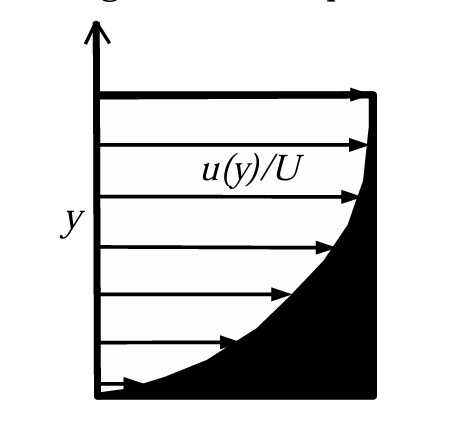
\includegraphics[width=0.3\columnwidth]{q8}
        \caption*{}
        \label{fig:q8}
    \end{figure}

    \begin{enumerate}
        \item boundary layer thickness.
        \item momentum thickness.
        \item displacement thickness.
        \item shape factor.
    \end{enumerate}

    \item The tangential velocity component 'V' of a spacecraft, which is in a circular orbit of radius 'R' around a spherical Earth ($\mu=GM \rightarrow$ gravitational parameter of Earth) is given by the following expression.
    \hfill{\brak{\text{AE 2018}}}

    \begin{enumerate}
        \begin{multicols}{2}
            \item $V=\sqrt{\frac{\mu}{2R}}$
            \item $V=\sqrt{\frac{\mu}{R}}$
            \item $V=\frac{2\pi}{\sqrt{\mu}}R^{\frac{3}{2}}$
            \item $V=\frac{2\pi}{\sqrt{\mu}}R^{\frac{2}{3}}$
        \end{multicols}
    \end{enumerate}

    \item Equation of the trajectory of a typical space object around any planet, in polar coordinates (r, $\theta$) (i.e. a general conic section geometry), is given as follows. (h is angular momentum, $\mu$ is gravitational parameter, e is eccentricity, r is radial distance from the planet center, $\theta$ is angle between vectors $\vec{e}$ and $\vec{r}$).
    \hfill{\brak{\text{AE 2018}}}

    \begin{enumerate}
        \begin{multicols}{2}
            \item $r=\frac{(h^{2}/_{\mu})}{1-e \cos \theta}$
            \item $r=\frac{(h^{2}/\mu)}{e-\cos \theta}$
            \item $r=\frac{(h^{2}/_{\mu})}{1+e \cos \theta}$
            \item $r=\frac{(h^{2}/\mu)}{e+\cos \theta}$
        \end{multicols}
    \end{enumerate}

    \item In an elliptic orbit around any planet, the location at which a spacecraft has the maximum angular velocity is
    \hfill{\brak{\text{AE 2018}}}

    \begin{enumerate}
        \item apoapsis.
        \item periapsis.
        \item a point at $+45^{\circ}$ from periapsis.
        \item a point at $-90^{\circ}$ from apoapsis.
    \end{enumerate}

    \item The pitching moment of a positively cambered NACA airfoil about its leading edge at zero-lift angle of attack is
    \hfill{\brak{\text{AE 2018}}}

    \begin{enumerate}
        \item negative.
        \item positive.
        \item indeterminate.
        \item zero.
    \end{enumerate}

    \item In a low-speed wind tunnel, the angular location(s) from the front stagnation point on a circular cylinder where the static pressure equals the free-stream static pressure, is
    \hfill{\brak{\text{AE 2018}}}

    \begin{enumerate}
        \begin{multicols}{2}
            \item $\pm38^{\circ}$
            \item $\pm30^{\circ}$
            \item $\pm60^{\circ}$
            \item $0^{\circ}$
        \end{multicols}
    \end{enumerate}

    \item A thermocouple, mounted flush in an insulated flat surface in a supersonic laminar flow of air measures the
    \hfill{\brak{\text{AE 2018}}}

    \begin{enumerate}
        \item static temperature.
        \item temperature greater than static but less than total temperature.
        \item total temperature.
        \item temperature greater than total temperature.
    \end{enumerate}

    \item A shock wave is moving into still air in a shock tube. Which one of the following happens to the air?
    \hfill{\brak{\text{AE 2018}}}

    \begin{enumerate}
        \item static temperature increases, total temperature remains constant.
        \item static temperature increases, total temperature increases.
        \item static temperature increases, total temperature decreases.
        \item static pressure increases, total temperature remains constant.
    \end{enumerate}

    \item The highest limit load factor experienced by a civil transport aircraft is in the range
    \hfill{\brak{\text{AE 2018}}}

    \begin{enumerate}
        \begin{multicols}{2}
            \item 0.0-2.0
            \item 2.0-5.0
            \item 5.0-8.0
            \item 8.0-10.0
        \end{multicols}
    \end{enumerate}

    \item Determine the correctness or otherwise of the following statements, [a] and [r]:
    
    [a] A closed-section box beam configuration is used in aircraft wings.
    
    [r] Closed-section box beam configuration is capable of resisting torsional loads.
    \hfill{\brak{\text{AE 2018}}}

    \begin{enumerate}
        \item Both [a] and [r] are true and [r] is the correct reason for [a].
        \item Both [a] and [r] are true but [r] is not the correct reason for [a].
        \item Both [a] and [r] are false.
        \item [a] is true but [r] is false.
    \end{enumerate}

    \item The first law of thermodynamics is also known as conservation of
    \hfill{\brak{\text{AE 2018}}}

    \begin{enumerate}
        \begin{multicols}{2}
            \item mass.
            \item momentum.
            \item energy.
            \item species.
        \end{multicols}
    \end{enumerate}

    \item In an ideal gas turbine cycle, the expansion in a turbine is represented by
    \hfill{\brak{\text{AE 2018}}}

    \begin{enumerate}
        \begin{multicols}{2}
            \item an isenthalpic process.
            \item an isentropic process.
            \item an isobaric process.
            \item an isochoric process.
        \end{multicols}
    \end{enumerate}

    \item The determinant of the matrix $\myvec{1 & 1 & -1 \\ 2 & 1 & 0 \\ 3 & 1 & 1}$ is \underline{\hspace{2cm}} \brak{\text{accurate to one decimal place}}.
    \hfill{\brak{\text{AE 2018}}}

    \item The theoretical maximum velocity \brak{in m/s} of air expanding from a reservoir at 700 K is \underline{\hspace{2cm}} \brak{\text{accurate to two decimal places}}. Specific heat of air at constant pressure is 1005 J/\brak{kg-K}.
    \hfill{\brak{\text{AE 2018}}}

    \item For a damped single degree of freedom system with damping ratio of 0.1, ratio of two successive peak amplitudes of free vibration is \underline{\hspace{2cm}} \brak{\text{accurate to two decimal places}}.
    \hfill{\brak{\text{AE 2018}}}

    \item The natural frequency \brak{in rad/s} of the spring-mass system shown in the figure below is \underline{\hspace{2cm}} \brak{\text{accurate to one decimal place}}.
    \hfill{\brak{\text{AE 2018}}}
    
    \begin{figure}[H]
        \centering
        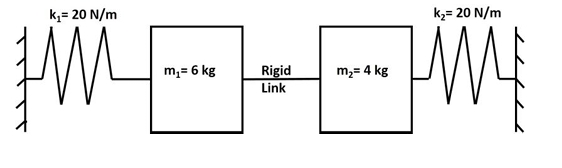
\includegraphics[width=0.8\columnwidth]{q23}
        \caption*{}
        \label{fig:q23}
    \end{figure}

    \item The stagnation pressures at the inlet and exit of a subsonic intake are 100 kPa and 98 kPa, respectively. The pressure recovery of this intake will be \underline{\hspace{2cm}} \brak{\text{accurate to two decimal places}}.
    \hfill{\brak{\text{AE 2018}}}

    \item A combustor is operating with a fuel-air ratio of 0.03. If the stoichiometric fuel-air ratio of the fuel used is 0.06, the equivalence ratio of the combustor will be \underline{\hspace{2cm}} \brak{\text{accurate to two decimal places}}.
    \hfill{\brak{\text{AE 2018}}}

    \item The solution of the differential equation $\frac{d^{2}y}{dx^{2}}+3\frac{dy}{dx}=0$ given that $y=0$ and $\frac{dy}{dx}=1$ at $x=0$ is
    \hfill{\brak{\text{AE 2018}}}

    \begin{enumerate}
        \begin{multicols}{2}
            \item $x(1-e^{-3x})$
            \item $\frac{1}{3}(1-e^{-3x})$
            \item $\frac{1}{3}(1+e^{-3x})$
            \item $\frac{1}{3}xe^{\frac{-3x}{2}}$
        \end{multicols}
    \end{enumerate}

    \item The relation between pressure (p) and velocity (V) for a steady, isentropic flow at two points along a streamline is, (c is a constant)
    \hfill{\brak{\text{AE 2018}}}

    \begin{enumerate}
        \item $c(p_{2}^{\gamma}-p_{1}^{\gamma})=\frac{V_{1}^{2}}{2}-\frac{V_{2}^{2}}{2}$
        \item $c(p_{2}^{\frac{\gamma}{\gamma-1}}-p_{1}^{\frac{\gamma}{\gamma-1}})=\frac{V_{1}^{2}}{2}-\frac{V_{2}^{2}}{2}$
        \item $c(p_{2}^{\frac{\gamma-1}{\gamma}}-p_{1}^{\frac{\gamma-1}{\gamma}})=\frac{V_{1}^{2}}{2}-\frac{V_{2}^{2}}{2}$
        \item $c(p_{2}^{\gamma-1}-p_{1}^{\gamma-1})=\frac{V_{1}^{2}}{2}-\frac{V_{2}^{2}}{2}$
    \end{enumerate}

    \item A thin airfoil is mounted in a low-speed, subsonic wind tunnel, in which the Mach number is 0.1. At a point on the airfoil, the pressure coefficient is measured to be -1.2. If the flow velocity is increased such that the free-stream Mach number is 0.6, the pressure coefficient at the same point on the airfoil will approximately be:
    \hfill{\brak{\text{AE 2018}}}

    \begin{enumerate}
        \begin{multicols}{4}
            \item -3.5
            \item -2.9
            \item -1.5
            \item -0.75
        \end{multicols}
    \end{enumerate}

    \item A solid circular shaft of diameter d is under pure torsion of magnitude T. The maximum tensile stress experienced at any point on the shaft is
    \hfill{\brak{\text{AE 2018}}}

    \begin{enumerate}
        \begin{multicols}{2}
            \item $\frac{32T}{\pi d^{3}}$
            \item $\frac{16T}{\pi d^{4}}$
            \item $\frac{32T}{\pi d^{4}}$
            \item $\frac{16T}{\pi d^{3}}$
        \end{multicols}
    \end{enumerate}

    \item A clamped-clamped beam, subjected to a point load P at the midspan, is shown in the figure below. The magnitude of the moment reaction at the two fixed ends of the beam is
    \hfill{\brak{\text{AE 2018}}}
    
    \begin{figure}[H]
        \centering
        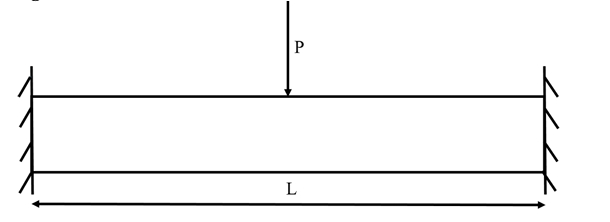
\includegraphics[width=0.8\columnwidth]{q30}
        \caption*{}
        \label{fig:q30}
    \end{figure}

    \begin{enumerate}
        \begin{multicols}{4}
            \item $PL/2$
            \item $PL/4$
            \item $PL/8$
            \item $PL/16$
        \end{multicols}
    \end{enumerate}

    \item Which of the following statement(s) is/are true about the state of a body in plane strain condition?
    
    P: All the points in the body undergo displacements in one plane only, for example the x-y plane, leading to $\epsilon_{zz}=\gamma_{xz}=\gamma_{yz}=0$
    
    Q: All the components of stress perpendicular to the plane of deformation, for example the x-y plane, of the body are equal to zero, i.e. $\sigma_{zz}=\tau_{xz}=\tau_{yz}=0$.
    
    R: Except the normal component, all the other components of stress perpendicular to the plane of deformation of the body, for example the x-y plane, are equal to zero, i.e. $\sigma_{zz}\ne0$, $\tau_{xz}=\tau_{yz}=0$.
    \hfill{\brak{\text{AE 2018}}}

    \begin{enumerate}
        \begin{multicols}{2}
            \item P only
            \item Q only
            \item P and Q
            \item P and R
        \end{multicols}
    \end{enumerate}

    \item An aircraft with a turbojet engine flies at a velocity of $100~m/s$. If the jet exhaust velocity is $300~m/s.$ the propulsive efficiency of the engine, assuming a negligible fuel-air ratio, is
    \hfill{\brak{\text{AE 2018}}}

    \begin{enumerate}
        \begin{multicols}{4}
            \item 0.33
            \item 0.50
            \item 0.67
            \item 0.80
        \end{multicols}
    \end{enumerate}

    \item An aircraft with a turboprop engine produces a thrust of 500 N and flies at $100~m/s$ If the propeller efficiency is 0.5, the shaft power produced by the engine is
    \hfill{\brak{\text{AE 2018}}}

    \begin{enumerate}
        \begin{multicols}{2}
            \item 50 kW
            \item 100 kW
            \item 125 kW
            \item 500 kW
        \end{multicols}
    \end{enumerate}

    \item An axial compressor that generates a stagnation pressure ratio of 4.0, operates with inlet and exit stagnation temperatures of 300 K and 480 K, respectively. If the ratio of specific heats ($\gamma$) is 1.4, the isentropic efficiency of the compressor is
    \hfill{\brak{\text{AE 2018}}}

    \begin{enumerate}
        \begin{multicols}{4}
            \item 0.94
            \item 0.81
            \item 0.72
            \item 0.63
        \end{multicols}
    \end{enumerate}

    \item A rocket has an initial mass of 150 kg. After operating for a duration of 10 s, its final mass is 50 kg. If the acceleration due to gravity is $9.81~m/s^{2}$ and the thrust produced by the rocket is 19.62 kN, the specific impulse of the rocket is
    \hfill{\brak{\text{AE 2018}}}

    \begin{enumerate}
        \begin{multicols}{2}
            \item 400 s
            \item 300 s
            \item 200 s
            \item 100 s
        \end{multicols}
    \end{enumerate}

    \item Consider the vector field $\vec{v}=-\frac{y}{r^{2}}\hat{i}+\frac{x}{r^{2}}j$; where $r=\sqrt{x^{2}+y^{2}}$. The contour integral $\oint \vec{v} \cdot \vec{ds}$, where $\vec{ds}$ is tangent to the contour that encloses the origin, is \underline{\hspace{2cm}} \brak{\text{accurate to two decimal places}}.
    \hfill{\brak{\text{AE 2018}}}

    \item The magnitude of the x-component of a unit vector at the point (1, 1) that is normal to equi-potential lines of the potential function $\phi(r)=\frac{1}{r^{2}+4}$, where $r=\sqrt{x^{2}+y^{2}}$ is \underline{\hspace{2cm}} \brak{\text{accurate to two decimal places}}.
    \hfill{\brak{\text{AE 2018}}}

    \item Assuming ISA standard sea level conditions (288.16 K, density of $1.225~kg/m^{3}$, $g=9.81{m/s}^{2}$, $R=287~J/(kg-K))$, the density (in $kg/m^{3}$) of air at Leh, which is at an altitude of 3500 m above mean sea level is \underline{\hspace{2cm}} \brak{\text{accurate to two decimal places}}.
    \hfill{\brak{\text{AE 2018}}}

    \item Consider a cubical tank of side 2 m with its top open. It is filled with water up to a height of 1 m. Assuming the density of water to be $1000~kg/m^{3}$, g as $9.81~m/s^{2}$ and the atmospheric pressure to be 100 kPa, the net hydrostatic force (in kN) on the side face of the tank due to the air and water is \underline{\hspace{2cm}} \brak{\text{accurate to two decimal places}}.
    \hfill{\brak{\text{AE 2018}}}

    \item An aircraft with mass of 400,000 kg cruises at $240~m/s$ at an altitude of 10 km. Its lift to drag ratio at cruise is 15. Assuming g as $9.81~m/s^{2}$, the power (in MW) needed for it to cruise is \underline{\hspace{2cm}} \brak{\text{accurate to two decimal places}}.
    \hfill{\brak{\text{AE 2018}}}

    \item A statically-stable aircraft has a ${C_{L_{\alpha}}}=5$ (where the angle of attack, $\alpha$, is measured in radians). The coefficient of moment of the aircraft about the center of gravity is given as $C_{M,c.g}=0.05-4\alpha$. The mean aerodynamic chord of the aircraft wing is 1 m. The location (positive towards the nose) of the neutral point of the aircraft from the center of gravity is \underline{\hspace{2cm}} (in m, accurate to two decimal places).
    \hfill{\brak{\text{AE 2018}}}

    \item An aircraft with a gross weight of 2000 kg, has a speed of $130~m/s$ at sea level, where the conditions are: 1 atmosphere (pressure), 288 K (temperature), and $1.23~kg/m^{3}$ (density). The speed (in m/s) required by the aircraft at an altitude of 9000 m, where the conditions are: 0.31 atmosphere, 230 K, and $0.47~kg/m^{3}$ to maintain a steady, level flight is \underline{\hspace{2cm}} (accurate to two decimal places).
    \hfill{\brak{\text{AE 2018}}}

    \item A pitot probe on an aircraft in a steady, level flight records a pressure of $55,000~N/m^{2}$. The static pressure and density are $45,280~N/m^{2}$ and $0.6~kg/m^{3}$, respectively. The wing area and the lift coefficient are $16~m^{2}$ and 2, respectively. The wing loading (in $N/m^{2}$) on this aircraft is \underline{\hspace{2cm}} (accurate to one decimal place).
    \hfill{\brak{\text{AE 2018}}}

    \item A spacecraft forms a circular orbit at an altitude of 150 km above the surface of a spherical Earth. Assuming the gravitational parameter, $\mu=3.986\times10^{14}m^{3}/s^{2}$ and radius of earth, $R_{E}=6,400~km$ the velocity required for the injection of the spacecraft, parallel to the local horizon, is \underline{\hspace{2cm}} (accurate to two decimal places).
    \hfill{\brak{\text{AE 2018}}}

    \item Air at 50 kPa pressure and 400 K temperature flows in a duct at Mach 3.0. A part of the flow leaks through an opening on the duct wall into the ambient, where the pressure is 30 kPa. The maximum Mach number achieved in the discharge is \underline{\hspace{2cm}} (accurate to two decimal places). (Ratio of specific heats of air is $\gamma=1.4$).
    \hfill{\brak{\text{AE 2018}}}

    \item Consider a $20^{\circ}$ half-angle wedge in a supersonic flow at Mach 3.0 at standard sea-level conditions. If the shock-wave angle on the wedge is $36^{\circ}$, the Mach number of the tangential component of the flow post-shock is \underline{\hspace{2cm}} (accurate to two decimal places).
    \hfill{\brak{\text{AE 2018}}}

    \item The boundary layer thickness at the location of a sensor on a flat plate in an incompressible, laminar flow of air is required to be restricted to 1 mm for an effective measurement. If the flow velocity is 20 m/s with 1 bar pressure, 300 K temperature, and $1.789\times10^{-5}$ kg/(m-s) viscosity, the maximum distance (in mm) of the sensor location from the leading edge is \underline{\hspace{2cm}} (accurate to one decimal place).
    \hfill{\brak{\text{AE 2018}}}

    \item Gross weight of an airplane is 7000 N, wing area is 16 m2, and the maximum lift coefficient is 2.0. Assuming density at the altitude as 1.23 kg/m3, the stall speed (in m/s) of the aircraft is \underline{\hspace{2cm}} (accurate to two decimal places).
    \hfill{\brak{\text{AE 2018}}}

    \item A thin-walled tube with external radius of 100 mm and wall thickness of 2 mm, is fixed at one end. It is subjected to a compressive force of 1 N acting at a point on the circumference parallel to its length. The maximum normal stress (in kPa) experienced by the structure is \underline{\hspace{2cm}} (accurate to two decimal places).
    \hfill{\brak{\text{AE 2018}}}

    \item A 1 m long massless cantilever beam oscillates at 2Hz, while a 60 kg mass is attached at the tip of it. The flexural rigidity of the beam (in kN-m2) is \underline{\hspace{2cm}} (accurate to two decimal places).
    \hfill{\brak{\text{AE 2018}}}

    \item A cantilever beam having a rectangular cross-section of width 60 mm and depth 100 mm, is made of aluminum alloy. The material mechanical properties are: Young's modulus, E = 73 GPa and ultimate stress, $\sigma_{u}$ = 480 MPa. Assuming a factor of safety of 4, the maximum bending moment (in kN-m) that can be applied on the beam is \underline{\hspace{2cm}} (accurate to one decimal place).
    \hfill{\brak{\text{AE 2018}}}

    \item The components of stress in a body under plane stress condition, in the absence of body forces, is given by: $\sigma_{xx} = Ax^{2}$; $\sigma_{yy} = 12x^{2} - 6y^{2}$ and $\sigma_{xy} = 12xy$. The coefficient, A, such that the body is under equilibrium is \underline{\hspace{2cm}} (accurate to one decimal place).
    \hfill{\brak{\text{AE 2018}}}

    \item An axial compressor rotor with 50 \% degree of reaction, operates with an axial velocity of 200 m/s. The absolute flow angle at the inlet of the rotor is 22o with reference to the axial direction. If the axial velocity is assumed to remain constant through the rotor, the magnitude of the relative velocity (in m/s) at the rotor exit is \underline{\hspace{2cm}} (accurate to one decimal place).
    \hfill{\brak{\text{AE 2018}}}

    \item The relative velocity of air leaving a straight radial impeller of a centrifugal compressor is 100 m/s. If the impeller tip speed is 200 m/s, for a slip free operation, the absolute velocity (in m/s) at the impeller exit is \underline{\hspace{2cm}} (accurate to one decimal place).
    \hfill{\brak{\text{AE 2018}}}

    \item An aircraft wind tunnel model, having a pitch axis mass moment of inertia (Iyy) of 0.014 kg-m2, is mounted in such a manner that it has pure pitching motion about its centre of gravity, where it is supported through a frictionless hinge. If the pitching moment (M) derivative with respect to angle of attack ($\alpha$), denoted by '$M_{\alpha}$', is -0.504 N-m/rad and the pitching moment (M) derivative with respect to pitch rate (q), denoted by 'Mq', is -0.0336 N-m/(rad/s), the damping ratio of the resulting motion due to an initial disturbance in pitch angle is approximately \underline{\hspace{2cm}} (accurate to three decimal places).
    \hfill{\brak{\text{AE 2018}}}

\end{enumerate}


\end{document}
